\documentclass[a1paper,portrait,margin=0.8cm]{baposter}

\usepackage{caption}
\usepackage{graphicx}
\usepackage{booktabs} % Horizontal rules in tables
\usepackage{relsize} % Used for making text smaller in some places
\usepackage{tikz}
\usepackage{amsmath,amsfonts,amssymb,amsthm} % Math packages
\usepackage{eqparbox}
\usepackage{lmodern}
\usepackage{xcolor}
\usepackage{textcomp}
\usepackage{enumitem}
\usepackage{microtype}
\usepackage{times}
\usepackage{cellspace}
\setlength{\tabcolsep}{1pt}


\setlist[itemize]{
    leftmargin=1em,
    itemindent=0em,
    labelindent=0.5em,
    labelsep=0.3em,
    topsep=0.2em,
    partopsep=0em,
    itemsep=0.1em,
    parsep=0.1em
}

\makeatletter
\renewenvironment{thebibliography}[1]{%
  \@ifundefined{chapter}{\section*{}{\relax}}{}
  \list{\@biblabel{\@arabic\c@enumiv}}%
    {\settowidth\labelwidth{\@biblabel{#1}}%
     \leftmargin\labelwidth
     \advance\leftmargin\labelsep
     \@openbib@code
     \usecounter{enumiv}%
     \let\p@enumiv\@empty
     \renewcommand\theenumiv{\@arabic\c@enumiv}}%
  \sloppy
  \clubpenalty4000
  \@clubpenalty \clubpenalty
  \widowpenalty4000%
  \sfcode`\.\@m}
  {\def\@noitemerr{\@latex@warning{Empty `thebibliography' environment}}%
  \endlist}
\makeatother

\usetikzlibrary{shapes.geometric, arrows, positioning}

% \tikzstyle{startstop} = [rectangle, rounded corners, minimum width=1.3cm, minimum height=1em,
%     text centered, draw=black, fill=purple!30,
%     font=\fontsize{3pt}{3pt}\selectfont,align=center]
% \tikzstyle{process} = [rectangle, minimum width=1.3cm, minimum height=1em,
%     text centered, draw=black, fill=purple!10,
%     font=\fontsize{3pt}{3pt}\selectfont,align=center]
% \tikzstyle{decision} = [diamond, aspect=2, minimum width=0.5cm, minimum height=1em,
%     text centered, draw=black, fill=purple!10,
%     font=\fontsize{3pt}{3pt}\selectfont,align=center]
% \tikzstyle{arrow} = [line width=0.1pt,->,>=stealth]


\definecolor{posterbg}{RGB}{173,215,220}
\definecolor{refbg}{RGB}{0,106,163}
\definecolor{bordercol}{RGB}{30,58,138} % Border color of content boxes
\definecolor{headercol1}{RGB}{200,246,224} % Background color for the header in the content boxes (left side)
\definecolor{headercol2}{RGB}{192,192,192} % Background color for the header in the content boxes (right side)
\definecolor{headerfontcol}{RGB}{0,170,255} % Text color for the header text in the content boxes
\definecolor{boxcolor}{RGB}{245,249,255} % Background color for the content in the content boxes
\definecolor{blockcolor}{RGB}{250,235,215}
\definecolor{subblockcolor}{RGB}{230,230,100}
\definecolor{Decision}{RGB}{255,203,183}


\begin{document}

\background{
\begin{tikzpicture}[remember picture,overlay]
\fill[color=posterbg]
    (-10,15) rectangle (current page.south east)

\shade[top color=white, bottom color=posterbg]
      (current page.north west) rectangle (30,15);

% \draw (current page.north west)+(-2em,2em) node[anchor=north west]
% {\includegraphics[height=1.1\textheight]{background}};
\end{tikzpicture}}


\begin{poster}{
columns=4,
colspacing=0.5em,
% rowspacing=0.1em,
grid=false,
borderColor=bordercol, % Border color of content boxes
headerColorOne=headercol1, % Background color for the header in the content boxes (left side)
headerColorTwo=headercol2, % Background color for the header in the content boxes (right side)
headerFontColor=headerfontcol, % Text color for the header text in the content boxes
boxColorOne=boxcolor, % Background color for the content in the content boxes
headershape=rounded, % Specify the rounded corner in the content box headers
headerfont=\small\rmfamily\bfseries, % Font modifiers for the text in the content box headers
textborder=rounded,
background=user,
headerborder=open, % Change to closed for a line under the content box headers
headerheight=0pt, 
boxheaderheight=1.2em,
boxpadding=6.5pt,
boxshade=plain,
linewidth=1.2pt,
textfont={\rmfamily \fontsize{5.5pt}{6.5pt}\selectfont}
}




\headerbox{}{name=titlebox, column=0, row=0, span=4,
boxColorOne=boxcolor,
headerColorOne=boxcolor,
headerColorTwo=boxcolor}{
\vspace*{-1.5em}
\centering

{\bfseries \huge\textcolor[RGB]{0,170,255}{Comparative Study and Optimization of SVD and CNN in Image Processing}}
\vspace*{-2em}

\begin{minipage}[b]{0.05\textwidth} 
\raggedleft
\includegraphics[scale=0.075]{SURF_LOGO.jpg}
\end{minipage}
\hfill
\begin{minipage}[b]{0.82\textwidth}
\raggedright
%{\bfseries \huge \textcolor{blue}{and No-SVD in Classification Tasks \\ }}
\begin{minipage}[b]{0.25\textwidth}
\footnotesize \textcolor{green}{\textbf{PROJECT CODE: \\}} SURF-2025-0145

\end{minipage}
\hfill
\begin{minipage}[b]{0.7\textwidth}
\vspace{-1em}
{\smaller \slshape Supervisor: Chi-Ru Yang } \\
{\smaller \slshape Members: Yang Fu, Yuhan Gong, Zhongting Hong, Shuyang Jin, Haohan Lin, Yuanchen Zhang} \\
{\smaller \slshape Volunteers: Siqing Cheng, Yifeng Shen, Jinhan Yang}
\end{minipage}
\end{minipage}
}
    


\headerbox{Abstract}{name=abstract,column=0,row=1,below=titlebox}{ 
\vspace{-0.7em}
Skin lesion image classification is pivotal for early dermatological diagnosis, yet traditional CNNs suffer from poor performance due to image noise and scarce annotated data.
\\This study proposes an SVD-enhanced CNN framework: SVD preprocesses ISIC 2019 images to suppress noise while preserving key lesion features. Combined with class weight optimization for data imbalance, it notably boosts skin lesion classification accuracy and robustness.


}


\headerbox{Introduction}{name=introduction,column=0,row=1,below=abstract}{
\vspace{-0.7em}
Cutaneous malignancies (e.g., malignant melanoma) severely threaten human health, and early accurate diagnosis is critical for improving patients’ survival rates. As a core of computer-aided diagnosis (CAD) systems, skin lesion image classification is indispensable for standardizing clinical screening and enhancing diagnostic efficiency, with datasets like ISIC 2019 providing large-scale annotated images for algorithm development.

Convolutional Neural Networks (CNNs) perform well in medical image recognition via robust feature extraction but have limitations in this task: image noise (e.g., hair artifacts) and scarce high-quality annotated data impair their ability to capture lesion features, leading to insufficient classification accuracy that fails to meet clinical needs.

Singular Value Decomposition (SVD) achieves signal-noise separation by preserving key feature-related components. Thus, this study proposes an SVD-enhanced CNN framework—integrating SVD into preprocessing to optimize input quality and combining class weight optimization to boost performance—with its accuracy validated on the ISIC 2019 dataset.


}



\headerbox{Summary \& Outlook}{name=summary,column=0,below=introduction}{ 
\vspace{-0.7em}
\noindent \textbf{Summary}\\
This study examined EfficientNet-B7 in skin lesion classification with Singular Value Decomposition (SVD) preprocessing. ISIC 2019 experiments showed SVD notably improved performance: training/validation accuracy (85\%/83\% vs. 78\%/75\% without SVD), loss (0.6/0.7 vs. 0.6/0.8), AUC (0.98/0.96 vs. 0.96/0.94), and more balanced precision/recall (\textasciitilde 0.8).


\noindent \textbf{Outlook}\\
Future work includes: optimizing SVD parameters for diverse lesions; combining SVD with other preprocessing methods; expanding datasets or using transfer learning for better generalization; and enhancing model interpretability to assist clinicians and facilitate clinical application.
}


\headerbox{Methodology}{name=methodology,column=1,below=titlebox,span=3}{
\vspace{-0.5em}
\begin{minipage}[b]{0.175\textwidth}
\noindent \textbf{Initial SVD Validation}\\
We first validated SVD on a small 4-class lung histopathology dataset using a lightweight pipeline:

\vspace{0.2em}
\begin{itemize}
    \item Preprocessing: $224 \!\times\! 224$ images with standard augmentation, per-channel SVD (fixed $k$=50, 100, 150 or auto-$k$, $\tau$=0.95), then normalization.
    \item Model: ResNet-18 trained with AdamW $\&$ early stopping.
    \item Result: SVD boosted test accuracy from 77.78\% to >92\%, with $k$=100, 150 being most stable.
\end{itemize}

\vspace{0.2em}
\noindent \textbf{Confusion Matrix}\\
We use the confusion matrix to visualize the test results to show which categories are mistakenly identified as which categories.

The rows represent the true categories, the columns represent the predicted categories, and the diagonal cells represent correct predictions, while the non-diagonal cells represent incorrect predictions.


\end{minipage}
\hfill
\begin{minipage}[b]{0.235\textwidth}

The absence of SVD shows obvious non-diagonal cells, indicating more confusion between categories.\\
When using SVD (with $k$ fixed at 100), the diagonal becomes stronger, the non-diagonal cells shrink, suggesting higher accuracy for each category and less confusion.

\centering
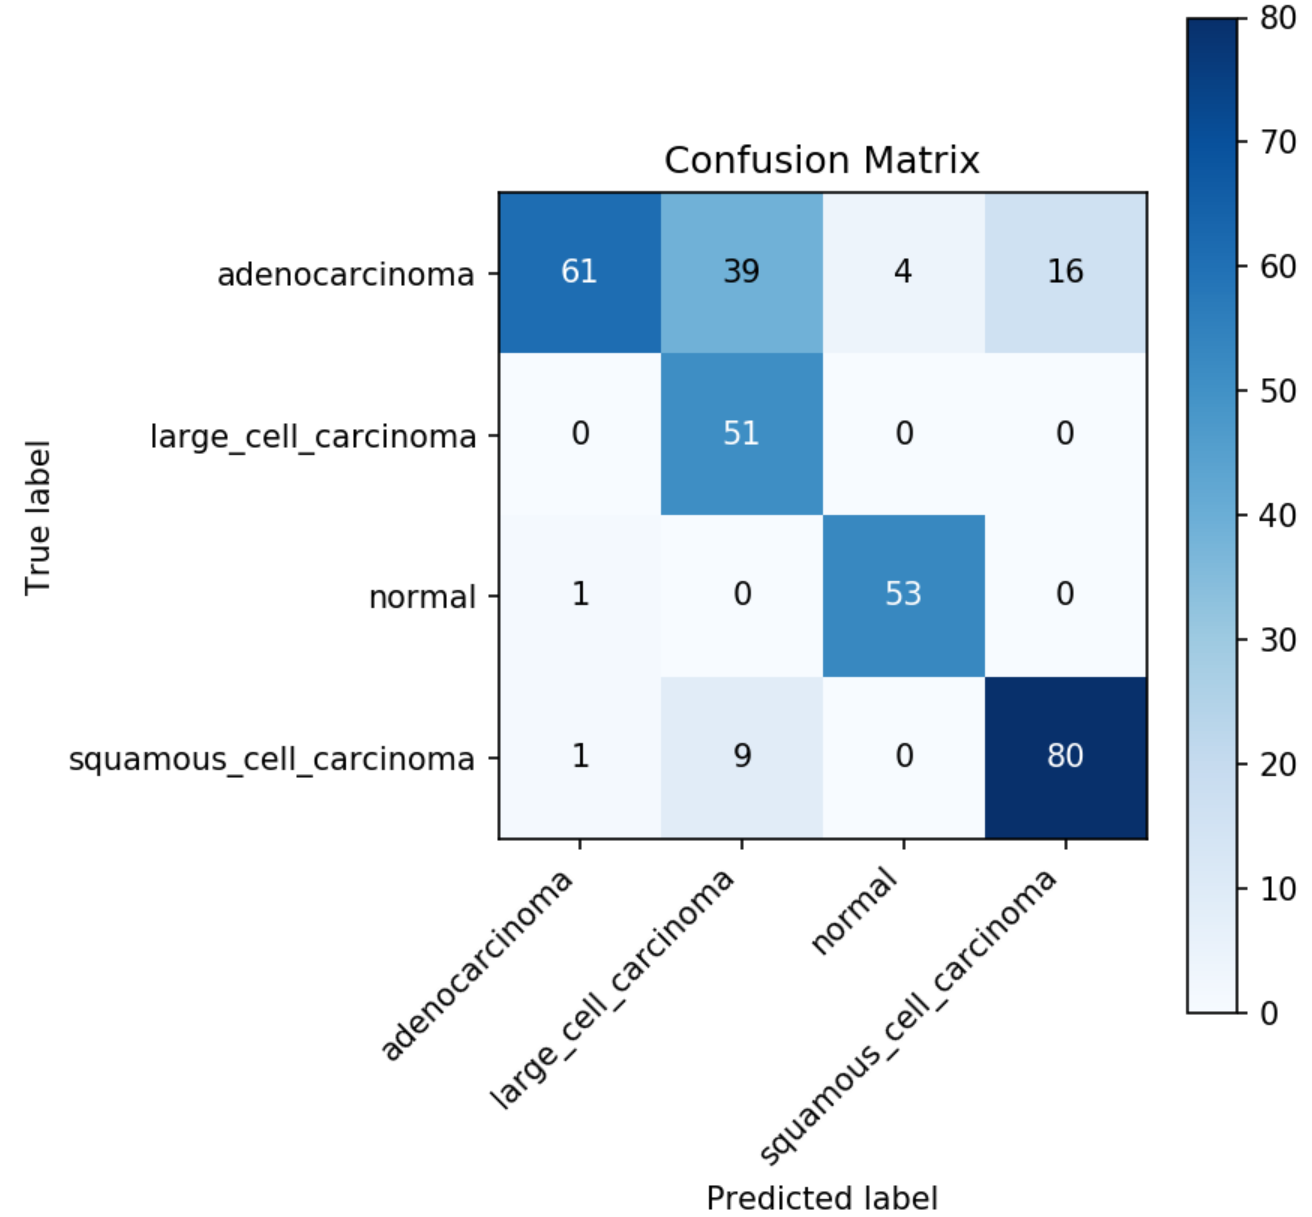
\includegraphics[width=0.95\linewidth]{confusion matrix.png} 

\vspace{-0.3em}
\textbf{Confusion Matrix \\ without SVD}
\vspace{0.7em}

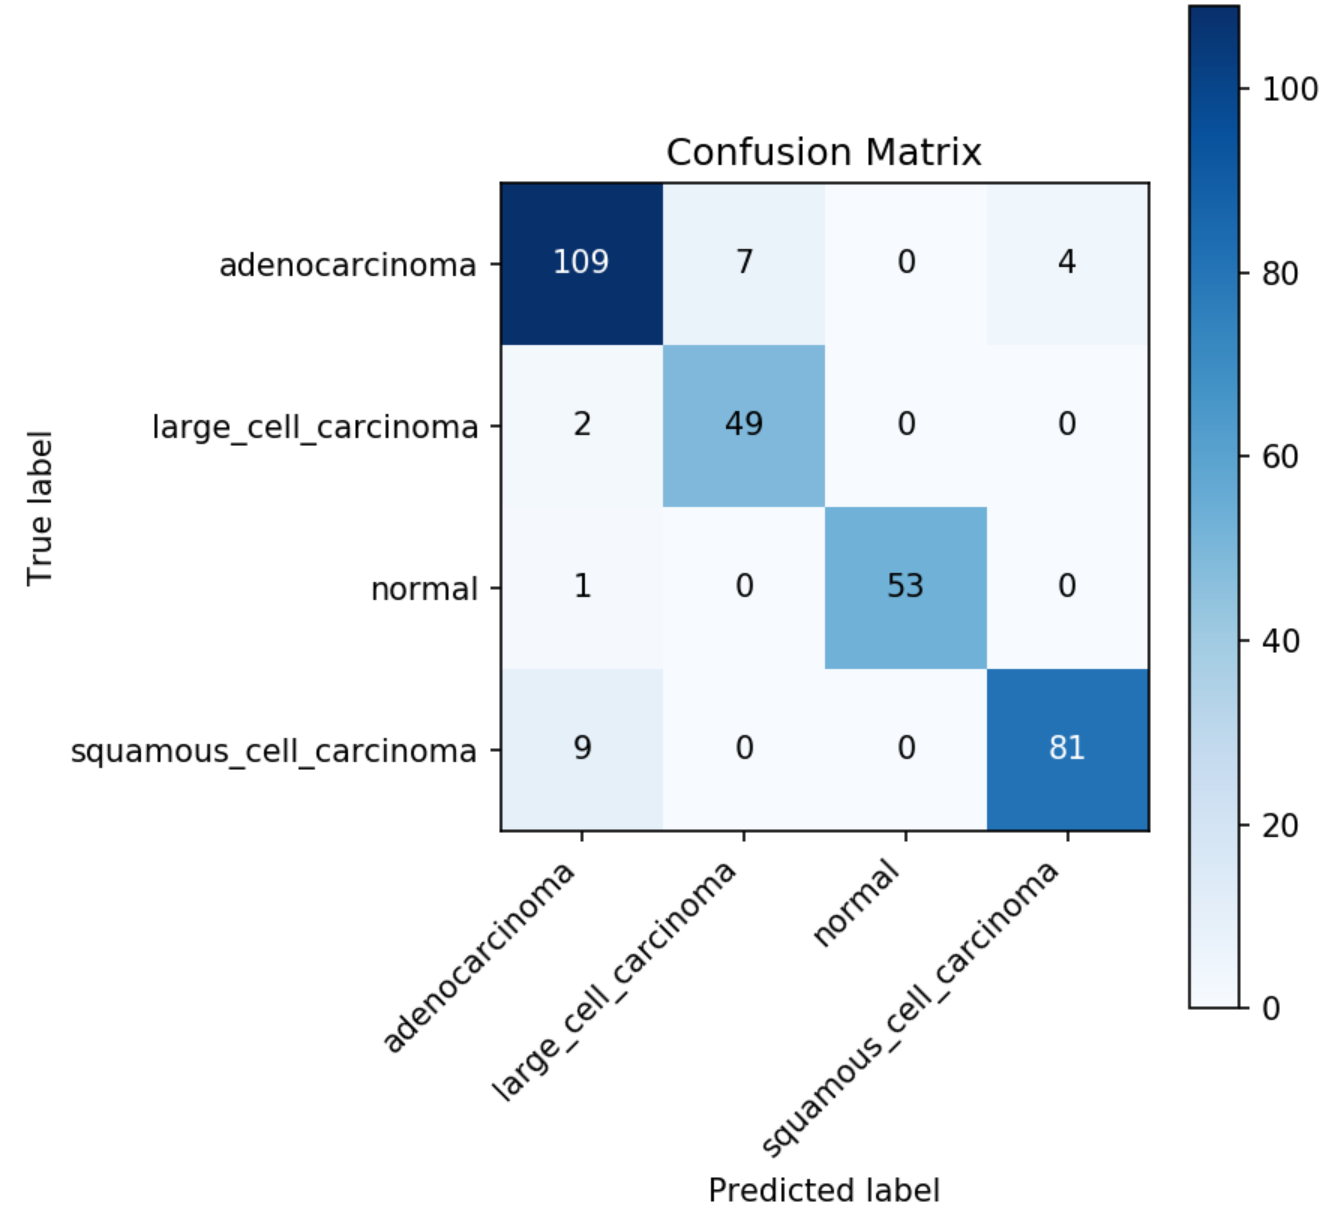
\includegraphics[width=0.95\linewidth]{confusion matrix (svd).png} 

\vspace{-0.3em}
\textbf{Confusion Matrix \\ with $k$=100 SVD}

\vspace{-0.3em}

\end{minipage}
\hfill
\begin{minipage}[b]{0.56\textwidth}

\noindent \textbf{Large-Scale Evaluation (ISIC 2019 Skin Lesion Dataset)}

\begin{minipage}[b]{0.46\textwidth}

\textbf{Preprocessing}
\begin{itemize}
    \item Color Handling: $BGR\!\rightarrow\! RGB$, LAB split; CLAHE (clip=3.0, grid=$8\!\times\!8$) on L channel + bilateral filtering (kernel=9, $\sigma$=75).
    \item Standardization: Resize to $384\!\times\!384$, normalize [0,1].
    \item Cache: NumPy arrays stored for reuse.
\end{itemize}
\vspace{0.2em}

\noindent \textbf{SVD Processing}\\
Using PyTorch, the model based on EfficientNet-B7 has two parts:
\vspace{0.2em}
\begin{itemize}
    \item Convert $RGB\!\rightarrow\! 3\!\times\!384\!\times\!384$, apply per-channel SVD ($k$=60), reconstruct, and revert to $384\!\times\!384\!\times\!3$.
\end{itemize}
\vspace{0.2em}

\noindent \textbf{Model}

\begin{itemize}
    \item Backbone: EfficientNet-B7 (ImageNet pretrained), adaptive pooling $\!\rightarrow\!$ 2560D features.
    \item Head: 4-layer FC ($2560\!\rightarrow\!1024\!\rightarrow\!512\!\rightarrow\!256\!\rightarrow\!7$) with SiLU, BatchNorm1d, Dropout(0.5).
\end{itemize}

\vspace{0.2em}

\noindent \textbf{Training}

\begin{itemize}
    \item Loss: Weighted cross-entropy (rare classes $\times$2–5).
    \item Optimizer: AdamW (lr=2e-5, wd=1e-5).
    \item Training: Gradient accumulation (batch=8$\rightarrow$32), dual schedulers (cosine + plateau), mixed precision, early stopping (15-epoch patience).
\end{itemize}

\end{minipage}
\hfill
\begin{minipage}[b]{0.5\textwidth}

\vspace{0.5em}

\textbf{Metrics} 

Accuracy, AUC, Precision, and Recall. Test outputs include probabilities and class distributions.

\centering
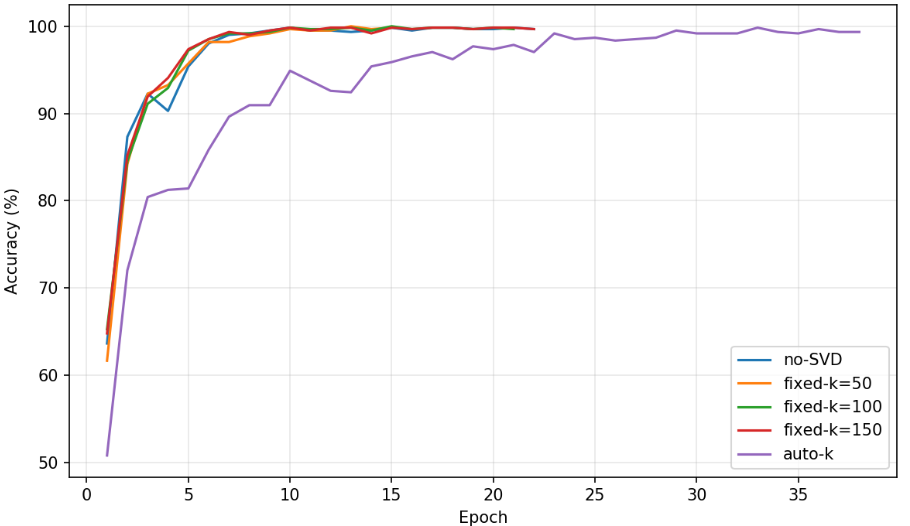
\includegraphics[width=0.96\linewidth]{train accuracy.png}

\vspace{-0.3em}
\textbf{Train Accuracy }
\vspace{0.5em}

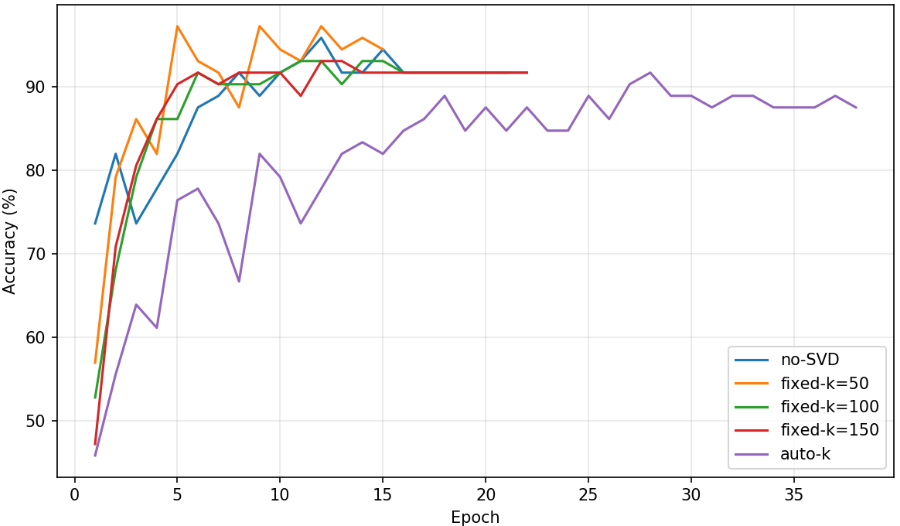
\includegraphics[width=0.96\linewidth]{validation accuracy.png}

\vspace{-0.3em}
\textbf{Validation Accuracy}
\vspace{0.5em}

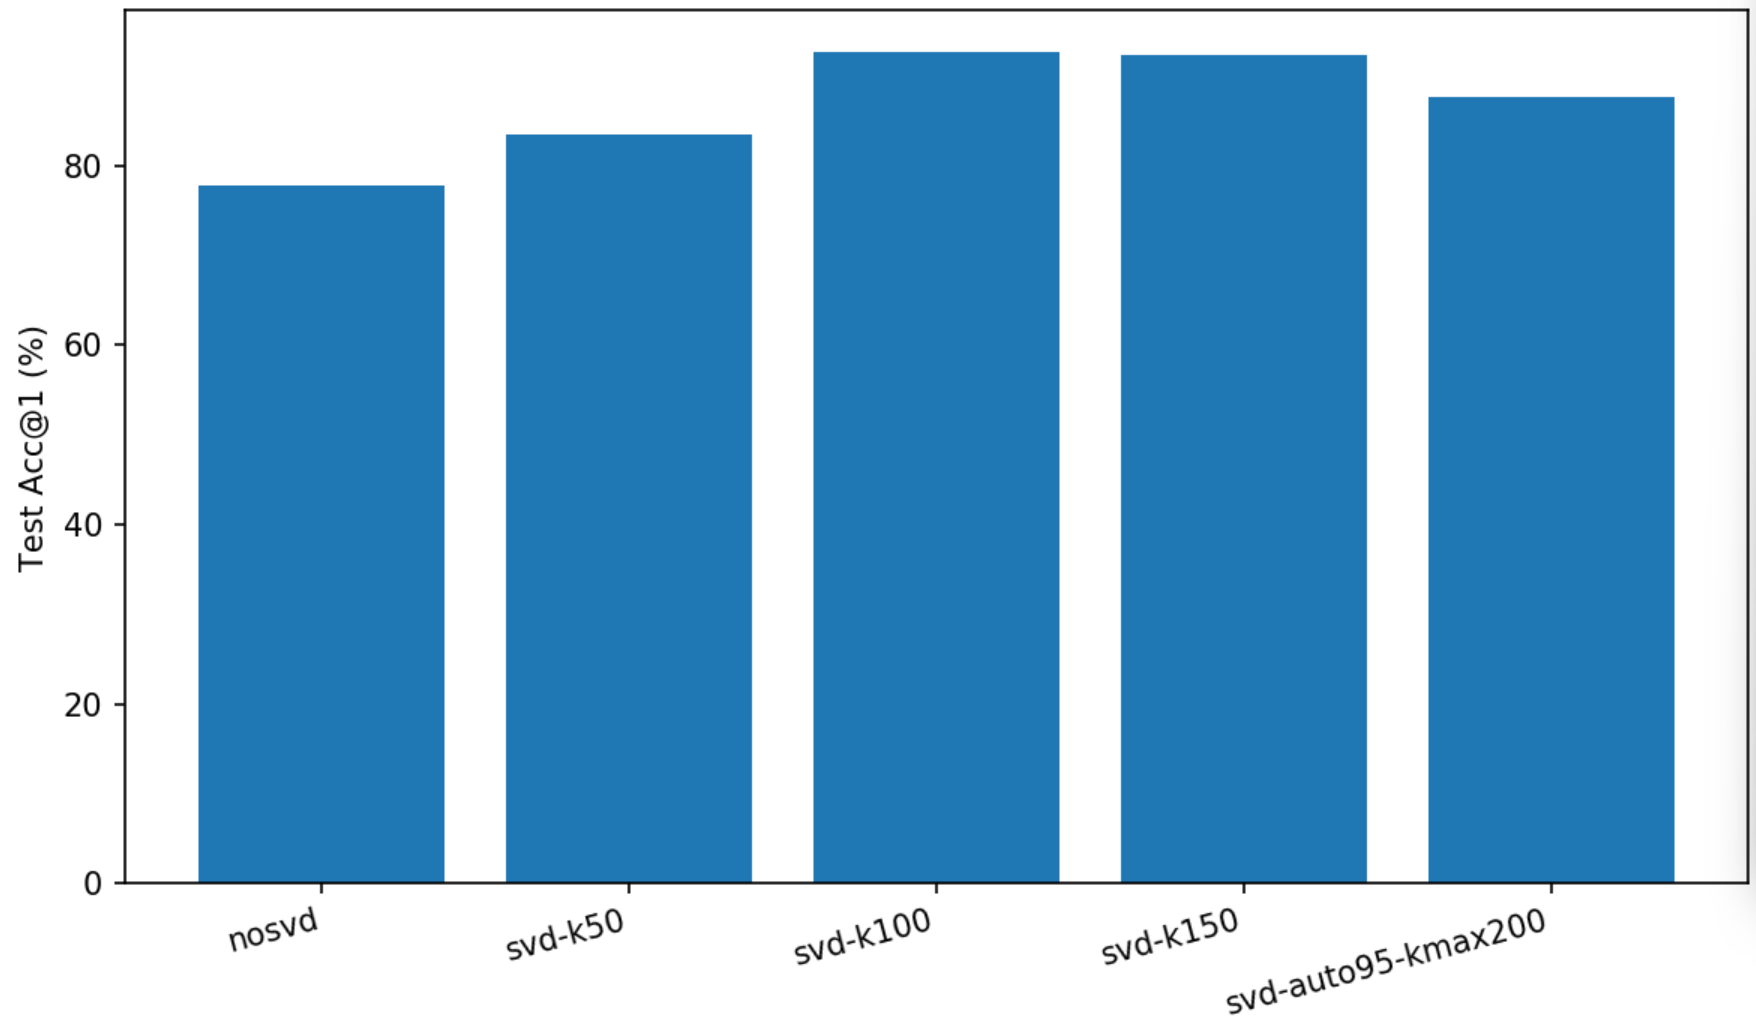
\includegraphics[width=0.96\linewidth]{test accuracy.png}

\vspace{-0.3em}
\textbf{Test Accuracy (Bar) }
\vspace{-0.5em}

\end{minipage}

\end{minipage}


}

\headerbox{\scriptsize Network Structure of Methodology}{name=structure,column=1,below=methodology}
{
\begin{minipage}[b]{\textwidth}

\vspace{-1em}

\centering
\begin{tikzpicture}[
    block/.style={rectangle, minimum width=1.3cm, minimum height=1.3em,
    text centered, draw=black, fill=blockcolor,
    font=\fontsize{4pt}{4pt}\selectfont,align=center},
    decision/.style={diamond, aspect=2, minimum width=0.1em, minimum height=0.1em,
    text centered, draw=black, fill=Decision,
    font=\fontsize{4pt}{4pt}\selectfont,align=center},
    line/.style={line width=0.3pt,->,>=stealth},
    subblock/.style={rectangle, minimum width=1.3em, minimum height=1.4em,
    text centered, draw=black, fill=subblockcolor,
    font=\fontsize{4pt}{4pt}\selectfont,align=center},
    nest/.style={draw, rounded corners, thick, inner xsep=3pt, inner ysep=2pt, fill=blockcolor},
    node distance=0.8em
]


% 左侧上层嵌套:Image Reading 相关
\node[nest] (img_nest) {
    \begin{tikzpicture}[node distance=0.8em]
        \node[subblock] (img_read) {Image Reading};
        \node[subblock, below=of img_read] (rgb_conv) {RGB Conversion};
        \node[subblock, below=of rgb_conv] (cont_enhance) {Contrast \\Enhancement};
        \draw[line] (img_read) -- (rgb_conv);
        \draw[line] (rgb_conv) -- (cont_enhance);
    \end{tikzpicture}
};

% Data Loading 及右侧输入
\node[block, above right=-0.3cm and 0.8cm of img_nest] (data_load) {Data Loading};

% Data Preprocessing
\node[block, below=of data_load] (data_pre) {Data Preprocessing};
\draw[line] (data_load) -- (data_pre);
\draw[line] (img_nest.east) |- (data_pre.west);

% SVD Denoising? 判断
\node[decision, below=of data_pre] (svd_denoise) {SVD \\ Denoising?};
\draw[line] (data_pre) -- (svd_denoise);

% 左侧 SVD 分支(YES 路径)
\node[block, below left=0.15cm and 1.2cm of svd_denoise] (calc_k) {Import $k$ Value};
\node[block, below=of calc_k] (gauss_blur) {Bilateral Filter};
\node[block, below=of gauss_blur] (resizing) {Resizing};
\draw[line] (svd_denoise.west) -- node[above]{\tiny Yes} ++(-3em,0) |- (calc_k.east);
\draw[line] (calc_k) -- (gauss_blur);
\draw[line] (gauss_blur) -- (resizing);

% Data Augmentation(NO 路径 及 左侧分支汇合)
\node[block, below=1em of svd_denoise] (data_aug) {Data Augmentation};
\draw[line] (svd_denoise.south) -- node[right]{\tiny No} (data_aug.north);
\draw[line] (resizing.east) -- ++(1.8em,0) |- (data_aug.west);

% Model Architecture
\node[block, below=of data_aug] (model_arch) {Model Architecture};
\draw[line] (data_aug) -- (model_arch);


% Model Training 及下方流程
\node[block, below=of model_arch] (model_train) {Model Training};
\draw[line] (model_arch) -- (model_train);

\node[block, below=of model_train] (model_val) {Model Validation};
\draw[line] (model_train) -- (model_val);

\node[block, below=of model_val] (perf_eval) {Model Evaluation};
\draw[line] (model_val) -- (perf_eval);

% 右侧模型结构嵌套:EfficientNet 相关
\node[nest, above left=-0.7cm and 0.8cm of perf_eval] (eff_nest) {
    \begin{tikzpicture}[node distance=0.8em]
        \node[subblock] (eff_back) {EfficientNet-B7 \\ Backbone};
        \node[subblock, below=of eff_back] (adap_pool) {Adaptive Pooling};
        \node[subblock, below=of adap_pool] (class_head) {Classifier Head};
        \draw[line] (eff_back) -- (adap_pool);
        \draw[line] (adap_pool) -- (class_head);
    \end{tikzpicture}
};
\draw[line] (eff_nest.east) -- ++(2.5em,0) |- (model_arch.west);

% 下方左侧嵌套:Weighted Loss 相关
\node[nest, below left=1.35cm and 0.8cm of model_train] (loss_nest) {
    \begin{tikzpicture}[node distance=0.8em]
        \node[subblock] (weight_loss) {Weighted Loss};
        \node[subblock, below=of weight_loss] (optimizer) {Optimizer};
        \node[subblock, below=of optimizer] (lr_sched) {Learning Rate\\ Scheduling};
        \draw[line] (weight_loss) -- (optimizer);
        \draw[line] (optimizer) -- (lr_sched);
    \end{tikzpicture}
};
\draw[line] (loss_nest.east) -- ++(3.5em,0) |- (model_train.west); 

% Early Stop? 判断
\node[decision, below=0.2cm of perf_eval] (early_stop) {Early Stop?};
\draw[line] (perf_eval) -- (early_stop);

% NO 路径(Test Inference 等)
\node[block, below=0.2cm of early_stop] (test_inf) {Test Inference};
\node[block, below=of test_inf] (res_vis) {Result Visualization};
\node[block, below=of res_vis] (return_res) {Return Result};
\draw[line] (early_stop.south) -- node[right]{\tiny No}  (test_inf.north);
\draw[line] (test_inf) -- (res_vis);
\draw[line] (res_vis) -- (return_res);


\draw[line] (early_stop.east) -- node[above]{\tiny Yes} ++(2em,0) |- (return_res.east);

\end{tikzpicture}

\vspace{-1.05em}

\end{minipage}
}

\headerbox{Core Background Knowledge}{name=svd,column=2,below=methodology,span=2}
{
\vspace{-0.7em}

\begin{minipage}[b]{0.5\textwidth}

\noindent \textbf{What is SVD} \\
SVD (Singular Value Decomposition) is a matrix factorization method in linear algebra used to decompose any matrix (whether square or not) into the product of three specific matrices. The mathematical form is: 
\vspace{-2em}
\begin{align*}
\mathbf{A} = \mathbf{U} \boldsymbol{\Sigma} \mathbf{V}^\text{T}
\end{align*}

\vspace{-2em}

$\mathbf{A}$: An $m \times n$ real or complex matrix. \\
$\mathbf{U}$: An $m \times m$ orthogonal matrix, known as the \emph{left singular vectors matrix}. \\
$\boldsymbol{\Sigma}$: An $m \times n$ diagonal matrix where the non- negative real numbers on its diagonal are called \emph{singular values}. \\
$\mathbf{V}^\text{T}$: The transpose of $\mathbf{V}$. $\mathbf{V}^\text{T} = \mathbf{V}^{-1}$ \\
$\mathbf{V}$ is an $n \times n$ orthogonal matrix  known as the \emph{right singular vectors matrix}.\\ 


\end{minipage}
\hfill
\begin{minipage}[b]{0.48\textwidth}

\noindent \textbf{The algebraic principles of SVD} \\
In essence, the process consists of a rotation, followed by a scaling operation, and then another rotation.

\vspace{-3em}
\setlength{\arraycolsep}{1.5pt}

% \[\!\!\!
% \!\begin{bmatrix} 2 & 1 \\ 1 & 2 \end{bmatrix} 
% \!\!\!=\!\!\!
% \begin{bmatrix} 
% \dfrac{1}{\sqrt{2}} & - \dfrac{1}{\sqrt{2}} \\[2pt]
% \dfrac{1}{\sqrt{2}} & \dfrac{1}{\sqrt{2}} 
% \end{bmatrix}\!\!\!
% \begin{bmatrix} 3 & 0 \\ 0 & 1 \end{bmatrix}\!\!\!
% \begin{bmatrix}
% \dfrac{1}{\sqrt{2}} & \dfrac{1}{\sqrt{2}} \\[2pt]
% - \dfrac{1}{\sqrt{2}} & \dfrac{1}{\sqrt{2}} 
% \end{bmatrix}
% \]

\[
\!\begin{bmatrix} 2 & 1 \\ 1 & 2 \end{bmatrix} 
\!\!=\!\!
\begin{bmatrix} 
\frac{1}{\sqrt{2}} & -\frac{1}{\sqrt{2}} \\[5pt]
\frac{1}{\sqrt{2}} & \frac{1}{\sqrt{2}} 
\end{bmatrix}\!\!
\begin{bmatrix} 3 & 0 \\ 0 & 1 \end{bmatrix}\!\!
\begin{bmatrix}
\frac{1}{\sqrt{2}} & \frac{1}{\sqrt{2}} \\[5pt]
-\frac{1}{\sqrt{2}} & \frac{1}{\sqrt{2}} 
\end{bmatrix}
\]

\vspace{-1.5em}

As shown in the figure, SVD can effectively achieve data compression in image processing. 

\begin{minipage}[b]{0.43\textwidth}
By retaining the top $k$ largest singular values, we can approximate the original matrix with significantly reduced data, leading to substantial storage savings. 
\end{minipage}
\hfill
\begin{minipage}[b]{0.55\textwidth}
    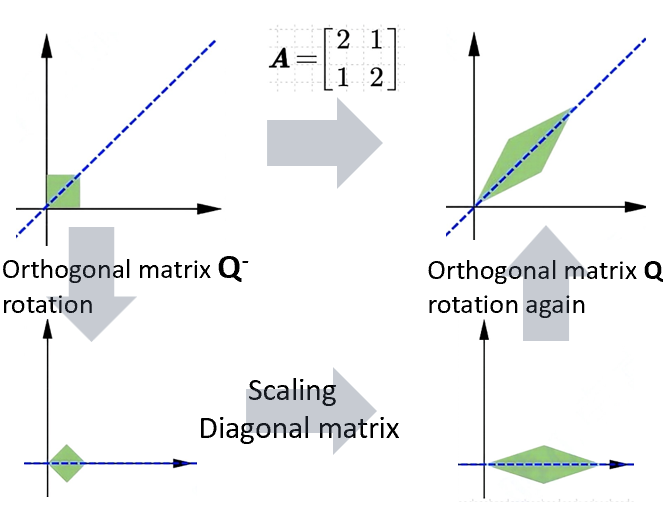
\includegraphics[width=\linewidth+1em]{SVD.jpg}
\end{minipage}

\vspace{-0.8em}

\end{minipage}
\hfill
\begin{minipage}[b]{0.65\textwidth}

\vspace{0.1em}

\noindent \textbf{Applications of SVD in Image Processing} \\

\vspace{-4em}

\setlength{\arraycolsep}{2pt}

\[
\boldsymbol{IM}\!
= \!\boldsymbol{PSQ}^\mathsf{T} \!
= (\boldsymbol{p}_1, \boldsymbol{p}_2, \ldots, \boldsymbol{p}_n)
\!\begin{bmatrix} \!
s_1 & 0 & 0 & 0 \\ 
0 & s_2 & 0 & 0 \\[-5pt]
\vdots & \vdots & \ddots & \vdots \\
0 & 0 & 0 & s_n 
\!\!\end{bmatrix}\!\!
\!\!\begin{bmatrix}
\boldsymbol{q}_1^\mathsf{T} \\[1pt]
\boldsymbol{q}_2^\mathsf{T} \\[-5pt] 
\vdots \\ 
\boldsymbol{q}_n^\mathsf{T} \!\!
\end{bmatrix}\!\!\!\!\!\!
\quad (s_1 \!\!>\!\! s_2 \!\!>\!\! s_3 \!\!>\!\! \cdots\!\! > \!\!s_n \!\!>\!\! 0)\!
\]
\vspace{-2em}
\[
\begin{aligned}
\boldsymbol{IM} \!
&= \!{s_1 \boldsymbol{p}_1 \boldsymbol{q}_1^\mathsf{T} 
\!+ \!s_2 \boldsymbol{p}_2 \boldsymbol{q}_2^\mathsf{T} 
\!+ \!s_3 \boldsymbol{p}_3 \boldsymbol{q}_3^\mathsf{T} 
\!+ \cdots +\! s_n \boldsymbol{p}_n \boldsymbol{q}_n^\mathsf{T}}_{\text{}}
\! = \!\boldsymbol{T}_1 \!+\! \boldsymbol{T}_2\! +\! \boldsymbol{T}_3 \!+ \cdots + \!\boldsymbol{T}_n
\end{aligned}
\]
\end{minipage}
% \hfill
% \begin{minipage}[b]{0.34\textwidth}

% \vspace{-3em}

% % 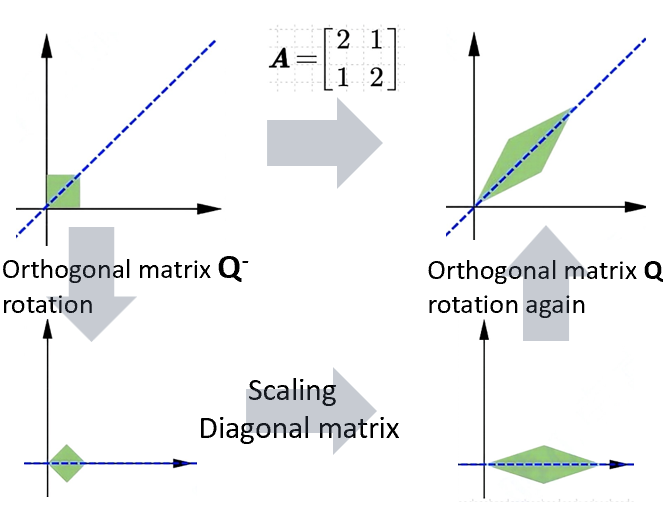
\includegraphics[width=\linewidth]{SVD.jpg}
% \end{minipage}

}


\headerbox{Results}{name=result,column=0,below=summary,span=4}{
\vspace{-0.6em}

    \begin{minipage}[t]{0.35\textwidth}  
    
        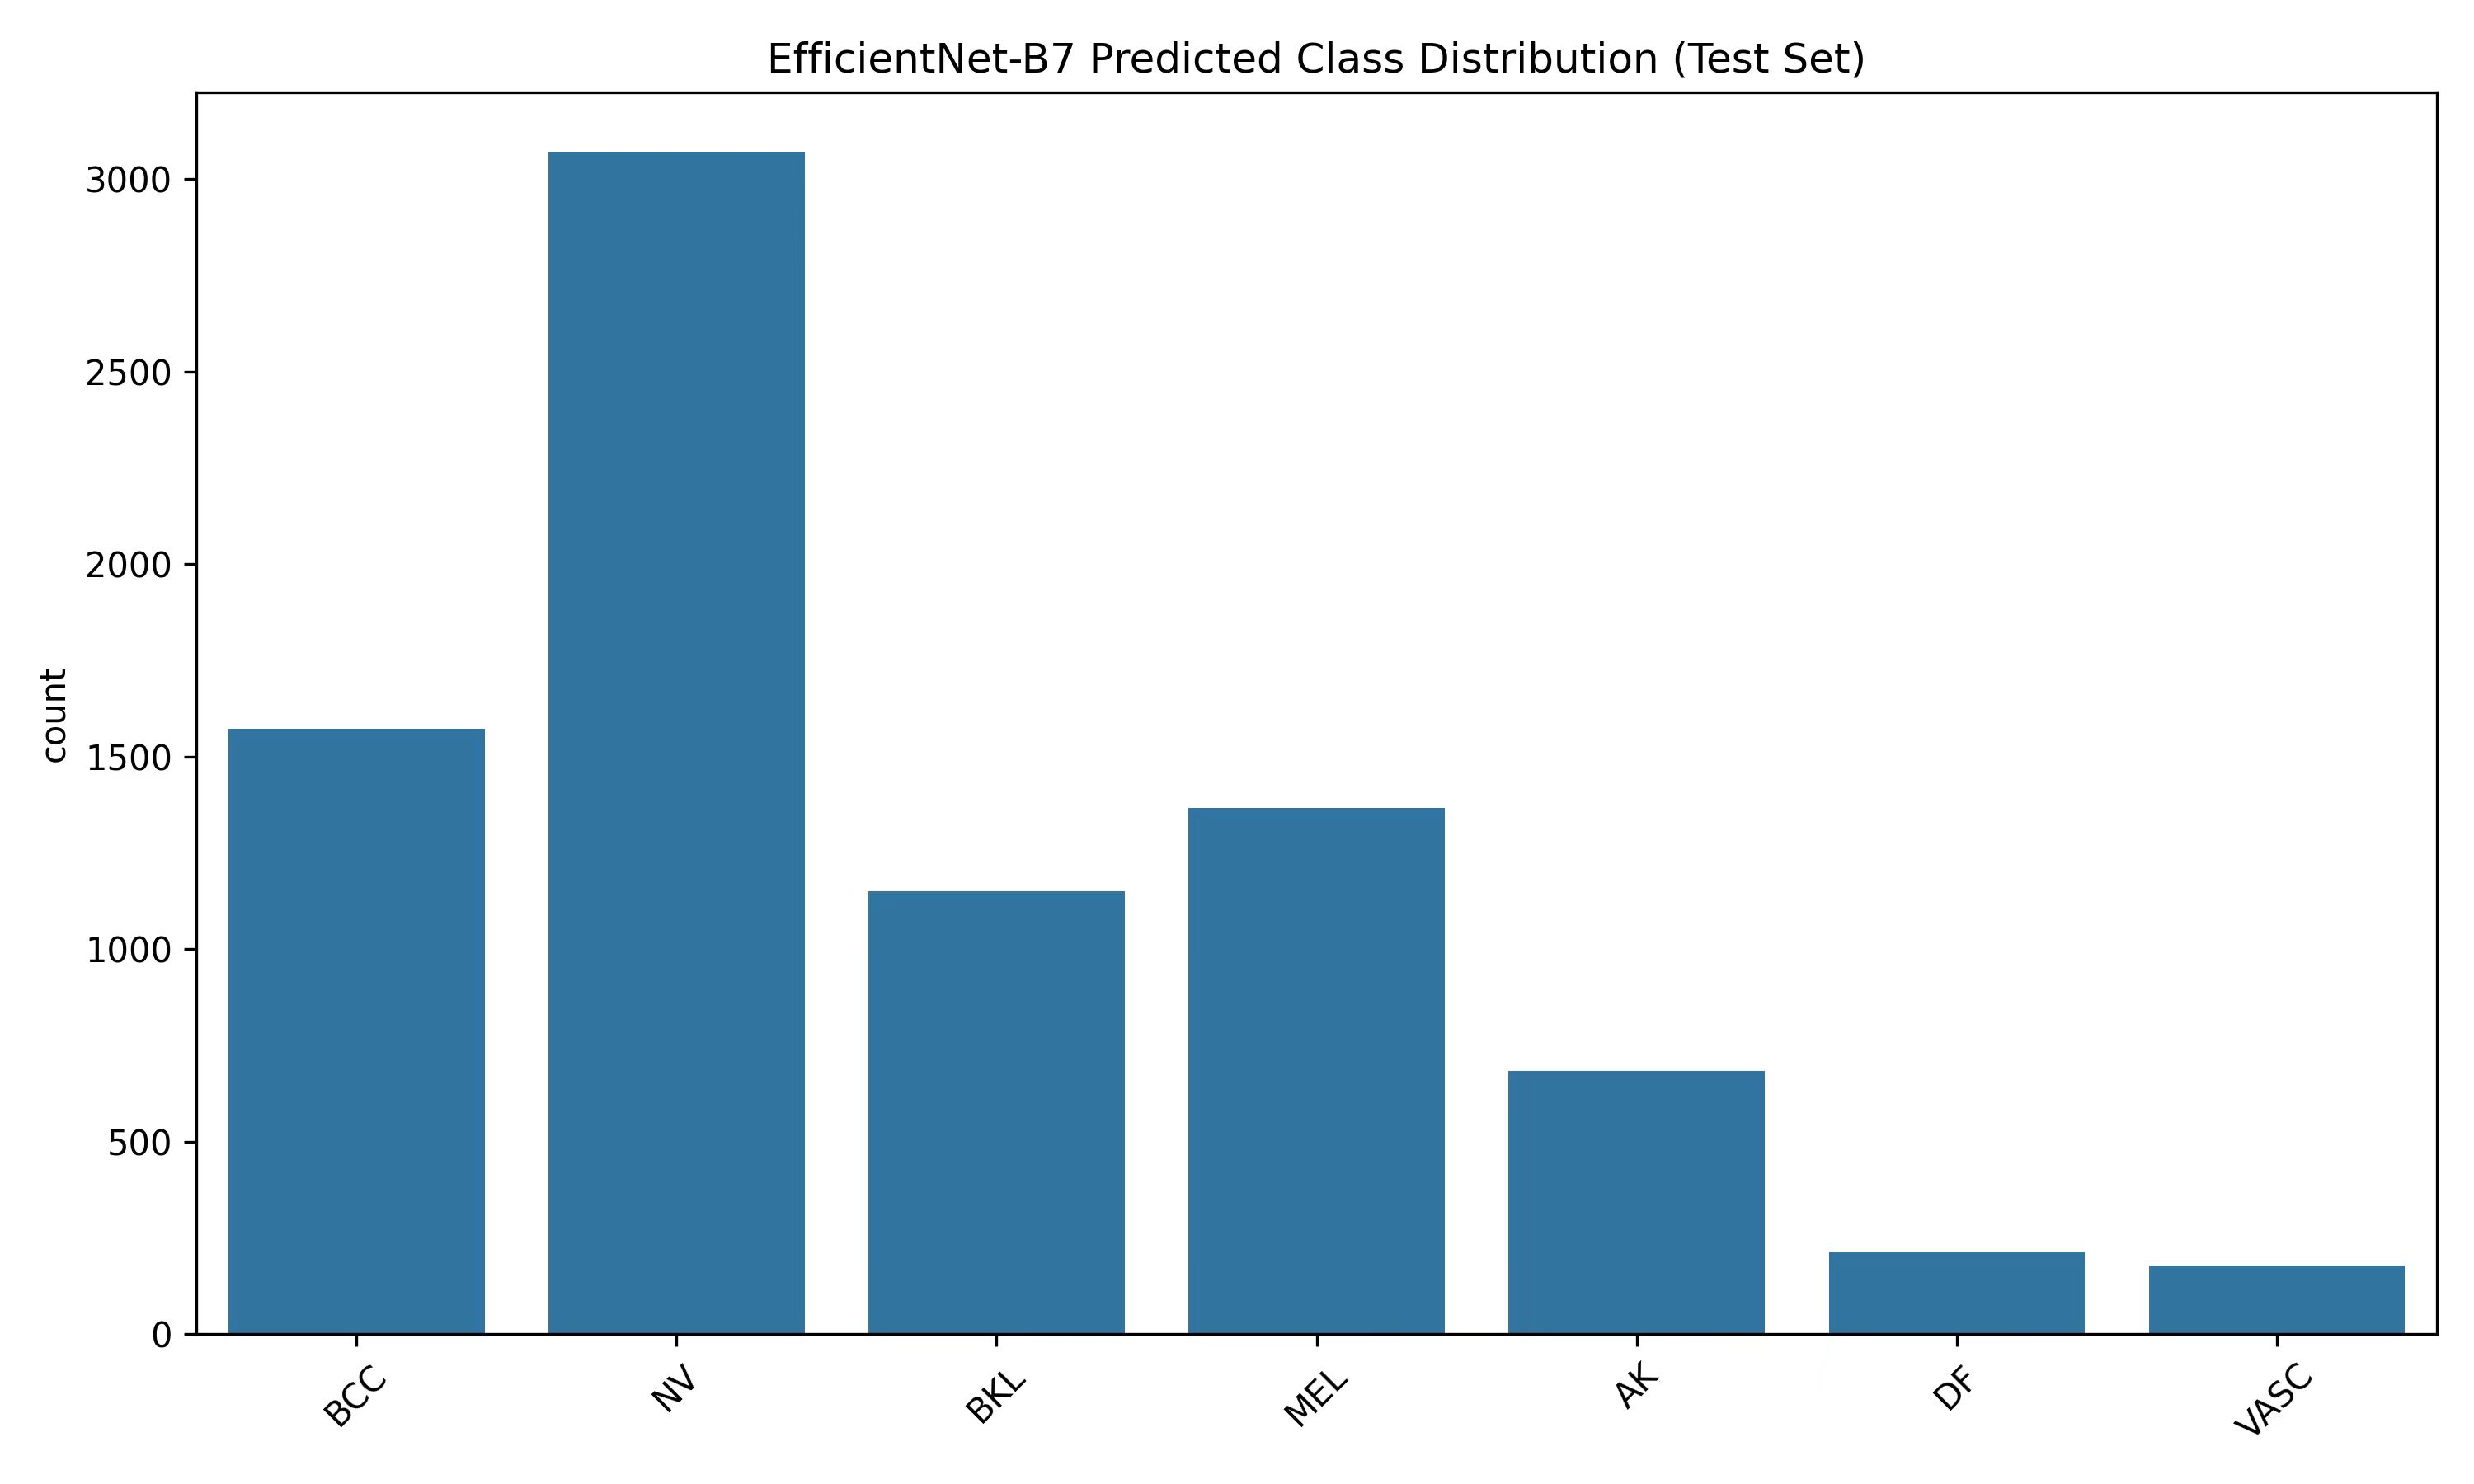
\includegraphics[width=\linewidth]{class distribution.jpg}
        \centering
        \textbf{Class Distribution} 
        
    \end{minipage}
    \hfill 
    \begin{minipage}[t]{0.315\textwidth} 
        
        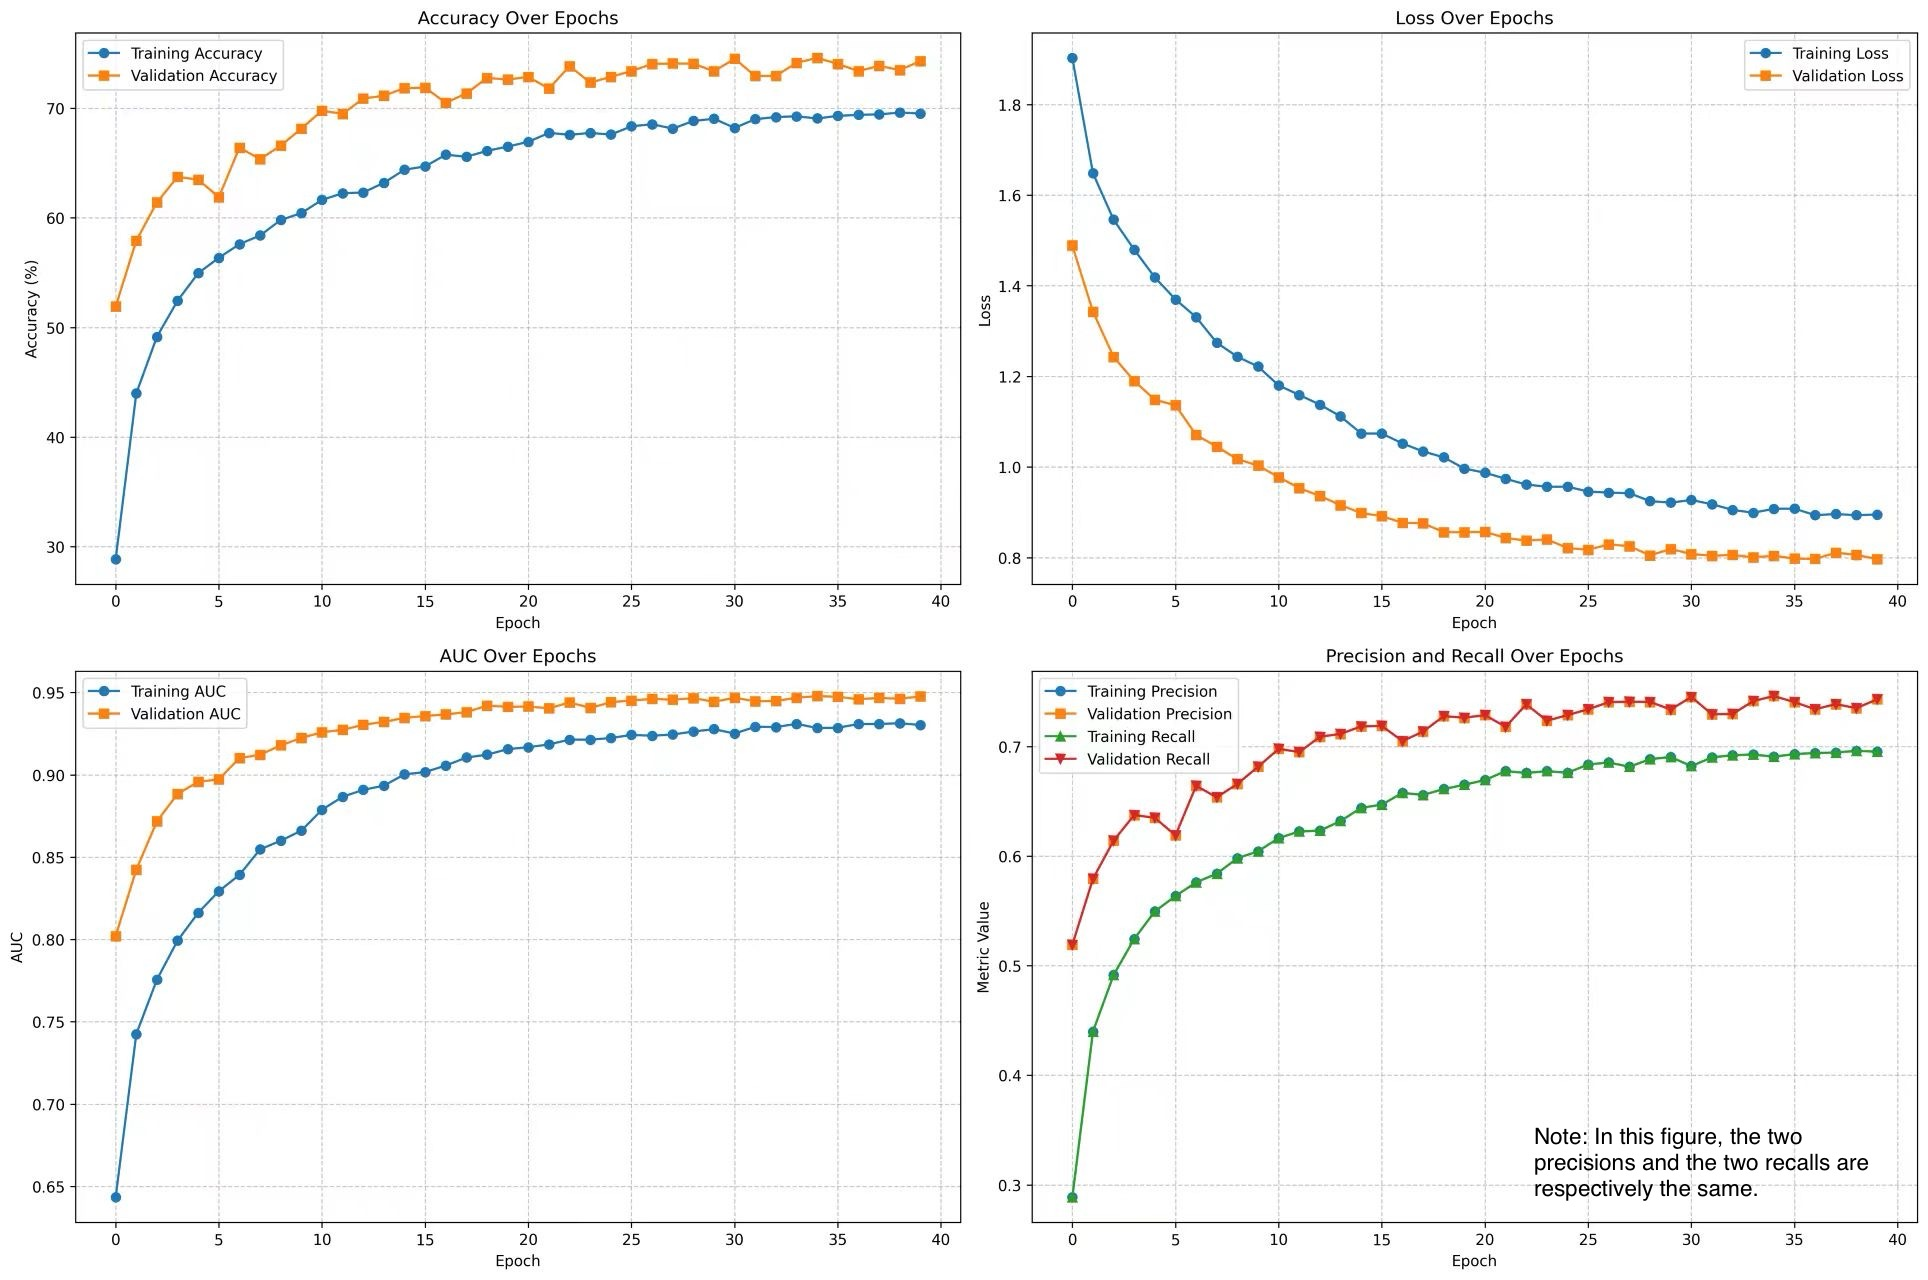
\includegraphics[width=\linewidth]{without svd.jpg}
        \centering
        \textbf{Without SVD} 
    \end{minipage}
    \hfill
    \begin{minipage}[t]{0.315\textwidth} 
        
        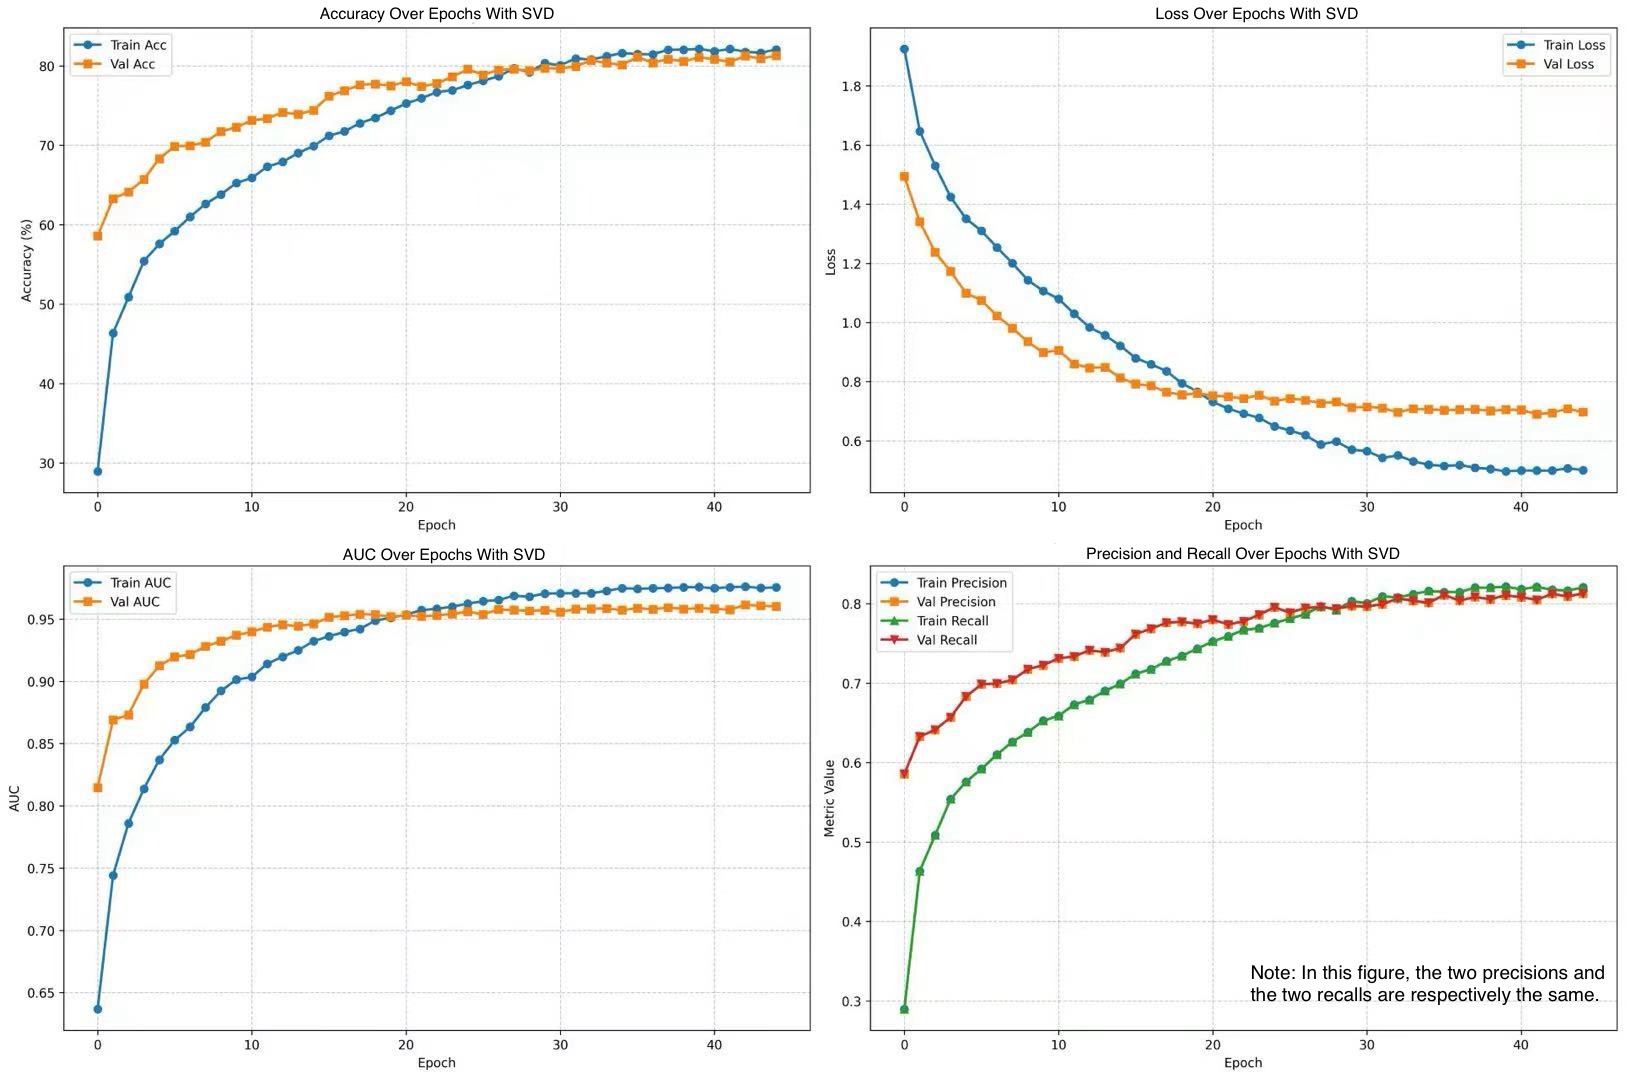
\includegraphics[width=\linewidth]{with svd.jpg}
        \centering
        \textbf{With SVD} 
    \end{minipage}

\vspace{-0.5em}
}

\headerbox{Selected References}{name=references,column=0,below=result,span=3,
headerborder=none,
headershape=rectangle,
textborder=none,above=bottom}
{

\begin{minipage}[t]{\linewidth}
\begin{tikzpicture}[remember picture,overlay]
\shade[left color=refbg, right color=white]
(-1.2em,3.5em) rectangle (\linewidth+1.2em, -5em) %height

\end{tikzpicture}

\vspace{-0.75cm}
\footnotesize\rmfamily\bfseries{Selected References\\}

\begin{minipage}[t]{\linewidth}
    \vspace{-2.4em}
    \fontsize{3pt}{3pt}\selectfont\mdseries
    % \setlength{\parskip}{0pt}  
    % \renewcommand{\bibitemsep}{0.01\baselineskip}
    % \setlength{\itemsep}{0.02\baselineskip}
    \nocite{*}
    \bibliographystyle{IEEEtran}
    \bibliography{biblio}
\end{minipage}
\end{minipage}

}

\headerbox{\scriptsize Contact Information}{name=info,column=3,below=result,headershape=rectangle,textborder=rectangle,boxheaderheight=1em,above=bottom}{

\vspace{-0.5em}
\hspace{-1em}
\begin{minipage}[b]{0.4\textwidth}
    
\begin{tabular}{S{c}|S{c}}

\begin{minipage}[t]{0.5\textwidth}
\vspace{-0.1em}
\centering
Project \\ QR Code
\end{minipage}
&
\begin{minipage}[t]{0.48\textwidth}
\vspace{-1em}
\includegraphics[width=\textwidth+1.6em]{qr_nobg.png}
\end{minipage}

\end{tabular}

\end{minipage}
\hfill
\begin{minipage}[b]{0.5\textwidth}
    
\begin{tabular}{S{c}|S{c}}

\begin{minipage}[t]{0.5\textwidth}
\vspace{-0.1em}
\centering
\hspace{0.4em} Poster \\ 
\hspace{0.4em} QR Code \\
\hspace{0.4em} (Details)
\end{minipage}
&
\begin{minipage}[t]{0.4\textwidth}
\vspace{-1em}
\includegraphics[scale=0.075]{QR.png}
\end{minipage}

\end{tabular}

\end{minipage}
}



\end{poster}

\end{document}